\documentclass[main.tex]{subfiles}
\begin{document}

\section{Given a stream of bits, how would you implement a parity bit to detect errors?}
Assume the following function signature in listing \ref{code:bitstream-parity-header} is available for use in the bitstream parity implementation. 

\lstinputlisting[caption={Bitstream Parity Header}, label={code:bitstream-parity-header}]{code/bitstream_parity/bitstream_parity.h}

\spoilerline
\subsection{Concept of Parity}
In digital communication, a parity bit is an extra bit appended to a binary data stream to assist in error detection. The goal is to keep the number of 1's in the data stream (including the parity bit) either even (\textit{even parity}) or odd (\textit{odd parity}), depending on the parity scheme. The \textit{parity} of a binary number refers to whether the number of 1's in the binary representation of the number is even or odd. Figure \ref{fig:parity-timing-dagiram} shows timing diagrams for no odd, and even parity, as well as even parity with an error. 

\begin{figure}[H]
    \centering
    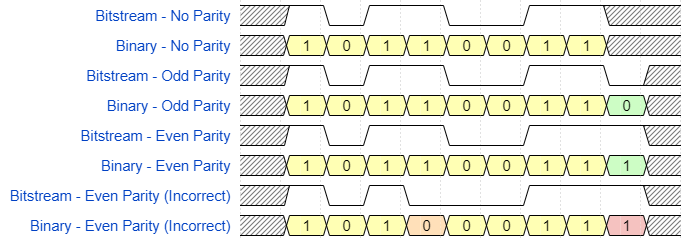
\includegraphics[scale=0.5]{images/parity.png}
    \caption{Parity Timing Diagram}
    \label{fig:parity-timing-dagiram}
\end{figure}

\subsection {Counting number of ones in a Byte}
To implement a parity bit, we need to count the number of 1's in the data stream\footnote{It's not uncommon to be asked this as a standalone question.}. 
\subsubsection{Bitwise Operations}
Before counting the number of \texttt{1}s in a byte, it’s important to understand bitwise operations. If you’re not familiar with these (ex: \&, |, >>, etc.), consider reviewing \bluehref{https://www.geeksforgeeks.org/bitwise-operators-in-c-cpp/}{Geeks for Geek's explanation on the topic}. Bitwise operations are common topics in embedded software interviews, and it's essential to understand them.

\subsubsection{Simple Approach}
A simple approach to count the number of 1's in a byte is to iterate through each bit and check if it's set. Listing \ref{code:count-one-simple} shows a simple implementation of this approach.

\lstinputlisting[caption={Simple Approach to Count Number of 1's in a Byte}, label={code:count-one-simple}]{code/bitstream_parity/count_ones_simple.c}

\noindent While effective, this approach is not efficient. It requires 8 iterations to count the number of 1's in a byte. We can improve this by using a technique called \textit{Brian Kernighan's Algorithm}.

\subsubsection{Brian Kernighan's Algorithm}
Brian Kernighan's Algorithm is a technique to count the number of set bits in a byte. The algorithm works by repeatedly 'removing' the least significant $1$ bit and counting the number of iterations required to reach 0. Listing \ref{code:count-one-brian-kernighan} shows the implementation of this algorithm. It is more efficient than the simple approach as it only requires the number of set bits to be counted \cite{seander_bithacks}.

\lstinputlisting[caption={Brian Kernighan's Algorithm to Count Number of 1's in a Byte}, label={code:count-one-brian-kernighan}]{code/bitstream_parity/count_ones_bk.c}

\subsubsection{Faster Ways}
There are faster ways to count the number of 1's in a byte, such as a lookup table to count the number of 1's for every byte. This approach is faster but requires more memory. Hamming Weight is another technique that counts the number of 1's in a byte in a more efficient manner, but it's more complex to implement (and usually out of scope for interviews). There's also usually a dedicated instruction, called popcount, that can count the number of set bits in one step, if supported by HW/compiler. More often than not, embedded interviews focus on the fundamentals and emphasize understanding over complex solutions.

\subsection{Implementing Parity Bit Check}
Putting it together, the steps to implement a parity bit are as follows:
\begin{itemize}
    \item For every byte, count the number of 1's (for this example, we'll use Brian Kernighan's Algorithm).
    \item Determine the expected parity bit based on the parity scheme (even or odd).
    \item Compare the parity bit to the expected parity bit.
\end{itemize}

\noindent Listing \ref{code:bitstream-parity} shows the implementation of the \texttt{check\_parity} function that implements the steps mentioned above.

\lstinputlisting[caption={Bitstream Parity Implementation}, label={code:bitstream-parity}]{code/bitstream_parity/bitstream_parity.c}

\end{document}